\documentclass[bachelor]{XJTUthesis}

\addbibresource[location=local]{reference//example.bib}

\begin{document}

% make cover
\titlenamea{西安交通大学}
\titlenameb{\LaTeX 毕业设计模板}
\xueyuan{电气学院}
\zhuanye{电气工程}
\banji{电气613}
\name{谢晋安}
\xuehao{0000000000}
\teacher{\LaTeX \quad GitHub}
\danwei{西安交通大学}
\cover

%\includepdf{xx.pdf} insert other pdf like this

\tableofcontents
\thispagestyle{empty}
\setcounter{page}{0}
\newpage

\begin{abstract}
这是一个模板。
\end{abstract}
\keywords{\LaTeX;XJTU}
\newpage
\begin{eabstract}
This is a template.
\end{eabstract}
\ekeywords{\LaTeX;XJTU}

\chapter{前言}
本模板针对西安交通大学毕业论文设计要求编写。可供需要完成毕业设计的同学使用。\par
本模板已经设置好页边距、页眉、页脚、字体等问题,符合毕业设计要求。

\chapter{用户手册}
\section{毕业论文撰写要求}
一篇完整的毕业论文或毕业设计说明书由封面、任务书、考核评议书、中文摘要、英文摘要、目录、正文(含结论)、致谢、参考文献、附录、封底等部分构成。正文字数不少于 15000 字(医、药类可根据学科特点,适当减少论文字数,但不得少于 10000 字),书写方式必须用计算机排版,白纸黑字双面打印,需要彩色打印的图例外\footnote{具体要求查看教务处网站}
\begin{enumerate}
  \item \textbf{题目}:即标题,它的主要作用是概括整篇论文的中心内容。因此,题目要确切、恰当、鲜明、简短,精炼。
  \item \textbf{摘要}:摘要是论文的高度概括,是全文的缩影,是长篇论文不可缺少的组成部分。要求用中、英文分别书写,一篇摘要不少于 400 字。英文摘要与中文摘要的内容和格式必须一致
  \item \textbf{目录}:反映论文的纲要。目录应列出通篇论文各组成部分的大小标题,分别层次,逐项标注页码,并包括注明参考文献、附录、索引等附属部分的页次,以便读者查找。
  \item \textbf{正文}:论文的正文是作者对自己的研究工作详细的表述。
  \item \textbf{参考文献}:文后著录的参考文献务必实事求是。论文中引用过的文献必须著录,未引用的文献不得出现。应遵循学术道德规范,避免涉嫌抄袭、剽窃等学术不端行为。
  \item \textbf{附录}:在论文之后附上不便放进正文的重要数据、表格、公式、图纸、程序等资料,供读者阅读论文时参考。附录不宜太多,附录的篇幅一般不要超过正文。
  \item \textbf{致谢}:对于毕业设计(论文)的指导教师,对毕业设计(论文)提过有益的建议或给予过帮助的同学、同事与集体,都应在论文的结尾部分书面致谢,言辞应恳切、实事求是。应注明受何种基金支持(没有可不写)。
\end{enumerate}

\section{本模板完成的设置}
纸张、页边距、页眉和页脚、三级标题的样式、正文字体行距、图题和表题、页码、封面、中英文摘要、目录、参考文献、附录、致谢。
\section{本模板提供的指令}
\subsection{封面页生成}

\begin{lstlisting}[language=tex]
\titlenamea{西安交通大学}
\titlenameb{\LaTeX 毕业设计模板}
\xueyuan{电气学院}
\zhuanye{电气工程}
\banji{电气613}
\name{谢晋安}
\xuehao{0000000000}
\teacher{\LaTeX \quad GitHub}
\danwei{西安交通大学}
\cover
\end{lstlisting}

\subsection{目录生成}
\subsection{中英文摘要}
\subsection{参考文献}
\subsection{附录和致谢}

\chapter{\LaTeX 强大的排版功能}
\section{微分算子及矢量运算}
\subsection{微分算子}
在直角坐标系中,哈密顿算子定义为\cite{冯慈璋2000工程电磁场导论}
\begin{equation}
    \nabla = \bm{e}_x\frac{\partial}{\partial x}+\bm{e}_y\frac{\partial}{\partial y}+\bm{e}_z\frac{\partial}{\partial z}
\end{equation}
为此,标量场$u(x,y,z)$的梯度可以写成
\begin{equation}
    grad u = \nabla u = \bm{e}_x\frac{\partial u}{\partial x}+\bm{e}_y\frac{\partial u}{\partial y}+\bm{e}_z\frac{\partial u}{\partial z}
\end{equation}
矢量$\bm{A}$的散度表示成
\begin{equation}
    div \bm{A} = \nabla\cdot\bm{A} = \frac{\partial A_x}{\partial x}+\frac{\partial A_y}{\partial y}+\frac{\partial A_z}{\partial z}
\end{equation}
矢量$\bm{A}$的旋度表示成
\begin{align}
\begin{split}
  rot \bm{A} & = \nabla\times\bm{A} =
  \left|
  \begin{array}{ccc}
    \bm{e}_x & \bm{e}_y & \bm{e}_z \\
    \frac{\partial}{\partial x} & \frac{\partial}{\partial y} & \frac{\partial}{\partial z} \\
    A_x & A_y & A_z
  \end{array}
  \right| \\
   & =\bm{e}_x \left(\frac{\partial A_z}{\partial y}-\frac{\partial A_y}{\partial z}\right)+\bm{e}_y \left(\frac{\partial A_x}{\partial z}-\frac{\partial A_z}{\partial x}\right)+\bm{e}_z \left(\frac{\partial A_y}{\partial x}-\frac{\partial A_x}{\partial y}\right)
\end{split}
\end{align}
\section{麦克斯韦方程组}
\begin{align}\label{maxwell}
  \nabla\times\bm{H} & =\bm{J}+\frac{\partial\bm{D}}{\partial t} \\
  \nabla\times\bm{E} & =-\frac{\partial\bm{B}}{\partial t} \\
  \nabla\cdot\bm{B} & =0 \\
  \nabla\cdot\bm{D} & =\rho
\end{align}

\chapter{TIKZ}
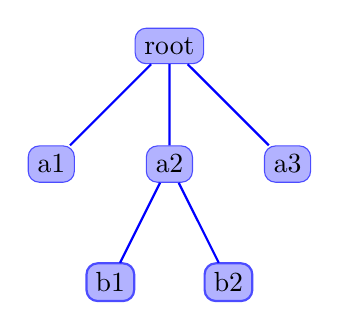
\begin{tikzpicture}
[every node/.style={fill=blue!30,draw=blue!70,rounded corners},
 edge from parent/.style={blue,thick,draw}]
    \node {root}
        child {node {a1}}
        child {node {a2}
            child {node {b1}}
            child {node {b2}}}
        child {node {a3}};
\end{tikzpicture}

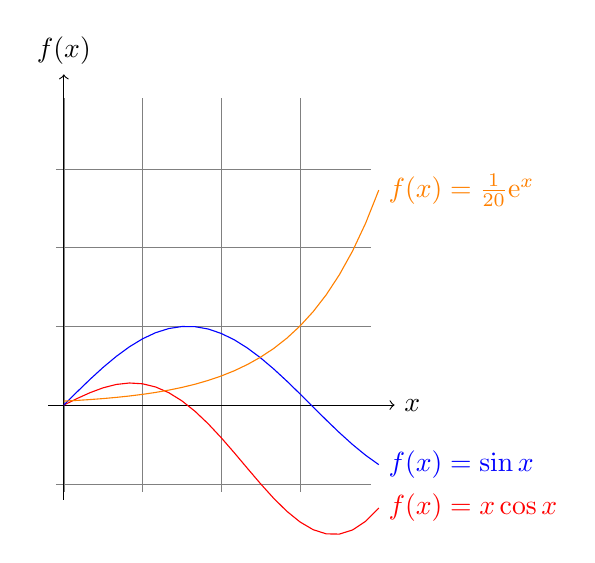
\begin{tikzpicture}[domain=0:4]
\draw[very thin,color=gray] (-0.1,-1.1) grid (3.9,3.9);
\draw[->] (-0.2,0) -- (4.2,0) node[right] {$x$};
\draw[->] (0,-1.2) -- (0,4.2) node[above] {$f(x)$};
\draw[color=red]    plot (\x,{0.5*\x*cos(\x r)})             node[right] {$f(x) =x\cos x$};
% \x r 表示弧度
\draw[color=blue]   plot (\x,{sin(\x r)})    node[right] {$f(x) = \sin x$};
\draw[color=orange] plot (\x,{0.05*exp(\x)}) node[right] {$f(x) = \frac{1}{20} \mathrm e^x$};
\end{tikzpicture}

\begin{tikzpicture}
    \graph {
        "$x_1$" -> "$x_2$"[red] -> "$x_3,x_4$";
        "$x_1$" ->[bend left] "$x_3,x_4$";
    };
\end{tikzpicture}


\chapter{一些环境}
表\ref{tab:test}是常用的三线表
\begin{table}[htbp]
    \centering
    \begin{tabular}{lcl}
        \toprule
        。。 & 。。 & 。。 \\
        \midrule
        。。 & 。。 & 。。 \\
        。。 & 。。 & 。。 \\
        。。 & 。。 & 。。 \\
        \bottomrule
    \end{tabular}
    \caption{\label{tab:test}示例表格}
\end{table}
algorithm环境
\begin{algorithm}
    \caption{Calculate $y = x^n$}
    \label{alg1}
    \begin{algorithmic}
        \REQUIRE $n \geq 0 \vee x \neq 0$
        \ENSURE $y = x^n$
        \STATE $y \leftarrow 1$
        \IF{$n < 0$}
        \STATE $X \leftarrow 1 / x$
        \STATE $N \leftarrow -n$
        \ELSE
        \STATE $X \leftarrow x$
        \STATE $N \leftarrow n$
        \ENDIF
        \WHILE{$N \neq 0$}
        \IF{$N$ is even}
        \STATE $X \leftarrow X \times X$
        \STATE $N \leftarrow N / 2$
        \ELSE[$N$ is odd]
        \STATE $y \leftarrow y \times X$
        \STATE $N \leftarrow N - 1$
        \ENDIF
        \ENDWHILE
    \end{algorithmic}
\end{algorithm}

lstlisting环境用于插入代码
\begin{lstlisting}[language=c++]
//hello.c
#include<stdio.h>
int main(void)
{
    int *p;
    printf("hello");
    return 0;
}
\end{lstlisting}

\begin{lstlisting}[language=matlab]
for i=1:100
    display('hello');
end
\end{lstlisting}

\chapter{杂项}

\begin{appendixs}
测试
\end{appendixs}

\begin{appendixs}
测试
\end{appendixs}

\begin{appendixs}
测试
\end{appendixs}

\begin{acknowledgement}
\chaptername
\end{acknowledgement}

\printbibliography[heading=bibliography,title=参考文献]
\end{document} 